\chapter{Implémentation}
        \section{Choix des technologies}
        Au cours de la réalisation d'un logiciel numérique,
        l'une des étapes les plus importantes est de choisir la bonne pile technologique. 
        Pourquoi? Parce qu'il s'agit de créer un produit qui ne consiste pas uniquement
        à concevoir une interface utilisateur agréable et une expérience utilisateur 
        pratique; il s'agit également de concevoir un produit stable, sécurisé et 
        maintenable qui, non seulement est en mesure de charmer les utilisateurs, mais vous 
        permettra également de faire évoluer l'entreprise.
        \paragraph{}
        Chaque couche de l'application est construite au-dessus d'une autre, 
        formant une pile. Cela rend les technologies Web fortement dépendantes 
        les unes des autres. L'image \ref{fig:pile} montre les principaux éléments constitutifs 
        d'une pile technologique typique; cependant, il peut y avoir d'autres éléments de 
        soutien impliqués.
        \begin{figure}[t]
                \centering
                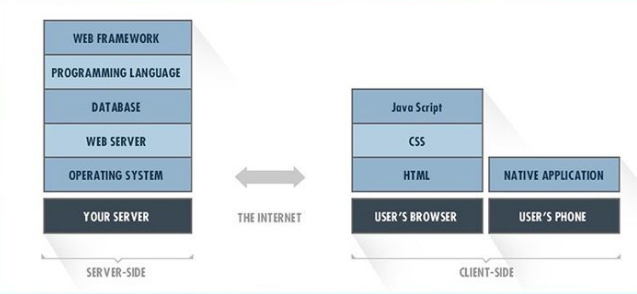
\includegraphics[scale=0.5]{images/Implementation/pile.png}
                \caption{Modèle du cycle de vie en cascade \cite{Bulatovych}}
                \label{fig:pile}
        \end{figure}
        \subsection{Frontend}
        L'interface utilisateur est également appelée côté client, car les utilisateurs voient et interagissent 
        avec cette partie d'une application. Pour une application web, cette interaction s'effectue 
        dans un navigateur web et est possible grâce à de nombreux outils de programmation. 
        Les applications Web destinées aux clients sont généralement créées à l'aide d'une combinaison 
        de JavaScript, HTML et CSS.
        \paragraph{Outils que nous utilisons pour le développement frontend:}
        \paragraph{}
        HTML (Hypertext Markup Language) est un langage de programmation utilisé pour décrire 
        la structure des informations présentées sur une page Web. 
        \subsection{Backend}
        \subsubsection{Application backend}
        \subsubsection{Base de données}
        \section{La hiérarchie dans l'application}
        \lipsum[1]
        \section{Ergonomie}
        % Interface utilisateur
        \lipsum[1]
        \section{Déploiement}
        \lipsum[1]
        \section{Sécurité du système}
        % -securitaire
        % -high reliability
        % -high scalability
        \lipsum[1]
        \section{Limitations du système}
        \lipsum[1]
        \section{Coûts}
        \lipsum[1]
    